\begin{frame}
\frametitle{late arriving packets (1)}
\begin{itemize}
\item suppose we transmit 1 bit per wallclock time unit:
\item wallclock time 0: A1 (1000 bit), A2 (500 bit)
\item wallclock time 800: B1 (250 bit), B2 (250 bit)
\vspace{.5cm}
\item want finish virtual times:
    \begin{itemize}
    \item A1 (1000), A2 (500)
    \item B1 (800 + 250), B2 (800 + 250)
    \end{itemize}
\item \ldots because we're on round 800 when B1, B2 received
\end{itemize}
\end{frame}

\begin{frame}
\frametitle{late arriving packets (2)}
\begin{itemize}
\item suppose we transmit 1 bit per wallclock time unit:
\item wallclock time 0: A1 (1000 bit), B1 (1100 bit)
\item wallclock time 800: C1 (500 bit)
\vspace{.5cm}
\item if we were going bit-by-bit we'd have transmitted 400 bits of A1 and 400 bits of B1
\item<2-> so we want finish virtual times:
    \begin{itemize}
    \item A1 (1000), B1 (1100), C1(\myemph{400}+500=900)
    \end{itemize}
\item<3-> problem: we can't stop transmitting A1 to transmit C1!
\end{itemize}
\end{frame}

\begin{frame}
\frametitle{tracking round numbers}
\begin{itemize}
\item N active queues $\implies$ virtual time speed is 1/Nth real time
    \begin{itemize}
    \item (plus need more adjustments for weights)
    \end{itemize}
\item if packets for A, B queued at time 0--100
    \begin{itemize}
    \item virtual time 0--100 (full speed)
    \end{itemize}
\item then packets for A, B, C queued at time 100-200
    \begin{itemize}
    \item virtual time 100--133 (one-third speed)
    \end{itemize}
\item if packets for B, C queued at time 200-400
    \begin{itemize}
    \item virtual time 133--183 (one-half speed)
    \end{itemize}
\item if packets for C queued at time 400-500
    \begin{itemize}
    \item virtual time 183-283 (full speed)
    \end{itemize}
\end{itemize}
\end{frame}


\begin{frame}
\frametitle{example}
\begin{itemize}
\item example: A1(1000 bit) @ 0, B1(900 bit) @ 500, C1(600 bit) @ 900, C2(100 bit) @ 2000, B2(200 bit) @ 2000\\
\begin{tabular}{lll}
wallclock time & virtual time & active packets (virt time, * = sending) \\
0              & 0         & A1 (1000*) \\
500            & 500       & A1 (1000*), B1 (1400) \\
900            & 700       & A1 (1000*), B1 (1400), C1 (1300) \\
1000           & 733       & B1 (1400*), C1 (1300) \\
1900           & 1183      & C1 (1300*) \\
2000           & 1283      & C1 (1300*), C2 (1400), B2 (1483) \\
\ldots         & \ldots    & \ldots \\
\end{tabular}
\end{itemize}
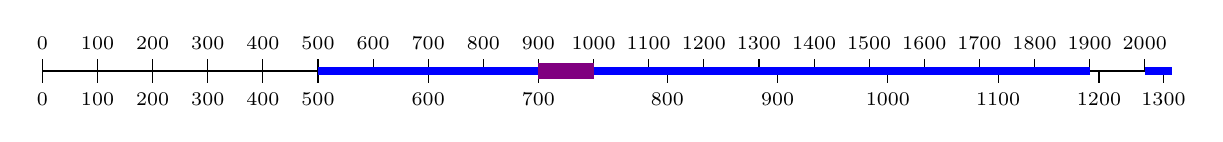
\begin{tikzpicture}
\begin{scope}[x=.7cm]
\draw (0, 0) -- (20.5, 0);
\foreach \x/\lbl in {0/0,1/100,2/200,3/300,4/400,5/500,6/600,7/700,8/800,9/900,10/1000,11/1100,12/1200,13/1300,14/1400,15/1500,16/1600,17/1700,18/1800,19/1900,20/2000} {
    \draw (\x, 0) -- ++(0,1.5mm) node[font=\scriptsize,above]{\lbl};
}
\foreach \x/\lbl in {0/0,1/100,2/200,3/300,4/400,5/500,7/600,9/700,11.34/800,13.34/900,15.34/1000,17.34/1100,19.17/1200,20.34/1300} {
    \draw (\x, 0) -- ++(0,-1.5mm) node[font=\scriptsize,below]{\lbl};
}
\draw[line width=1mm,blue] (5, 0) -- (9, 0);
\draw[line width=2mm,violet] (9, 0) -- (10, 0);
\draw[line width=1mm,blue] (10, 0) -- (19, 0);
\draw[line width=1mm,blue] (20, 0) -- (20.5, 0);
\end{scope}
\end{tikzpicture}
\end{frame}

